\section*{Evaluation}
We have done several sets of tests by using different size of data($machine$ x $job$), and we let the number of tasks equal to the number of jobs(tasks can be less than jobs). We use the data set retrieved from SAS web site[6], one of the test result is shown as follow:\\
\subsection*{Test result: 10x10}
Machine Number: 10,  Job Number: 10
\begin{itemize}
 
\item Job0: [(2,44),(3,5),(5,58),(4,97),(0,9),(7,84),(8,77),(9,96),(1,58),(6,89)],  

\item Job1: [(4,15),(7,1),(1,87),(8,57),(0,77),(3,85),(2,81),(5,39),(9,73),(6,21)],  

\item job2: [(9,82),(6,22),(4,10),(3,70),(1,49),(0,40),(8,34),(2,48),(7,80),(5,71)], 

\item job3: [(1,91),(2,17),(7,62),(5,75),(8,47),(4,11),(3,7),(6,72),(9,35),(0,55)], 

\item job4: [(6,71),(1,90),(3,75),(0,64),(2,94),(8,15),(4,12),(7,67),(9,20),(5,50)], 

\item job5: [(7,70),(5,93),(8,77),(2,29),(4,58),(6,93),(3,68),(1,57),(9,7),(0,52)],   

\item job6: [(6,87),(1,63),(4,26),(5,6),(2,82),(3,27),(7,56),(8,48),(9,36),(0,95)], 

\item job7: [(0,36),(5,15),(8,41),(9,78),(3,76),(6,84),(4,30),(7,76),(2,36),(1,8)], 

\item job8: [(5,88),(2,81),(3,13),(6,82),(4,54),(7,13),(8,29),(9,40),(1,78),(0,75)], 

\item job9: [(9,88),(4,54),(6,64),(7,32),(0,52),(2,6),(8,54),(5,82),(3,6),(1,26)]   

\end{itemize}

\begin{figure}[H]
\centering
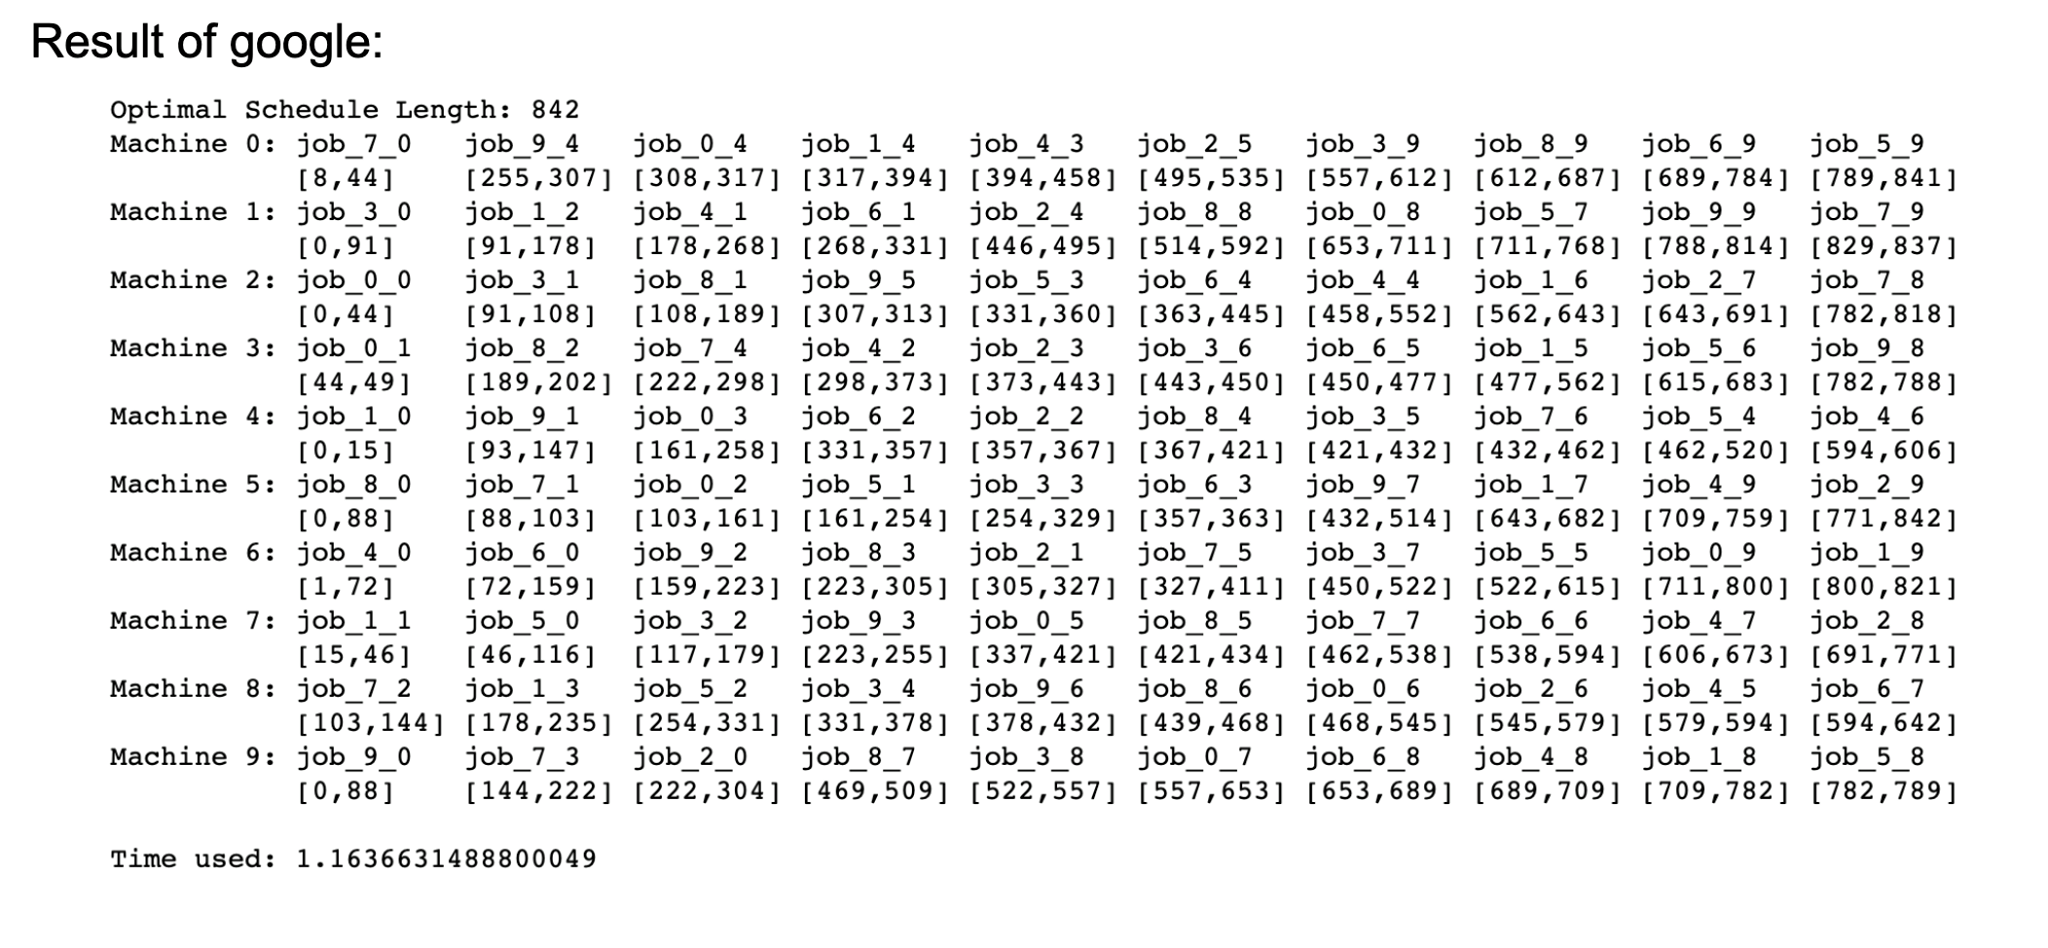
\includegraphics[width=4in]{img/google.png}
\caption{10x10 testing result of Google-OR-tool}
\end{figure}

\begin{figure}[H]
\centering
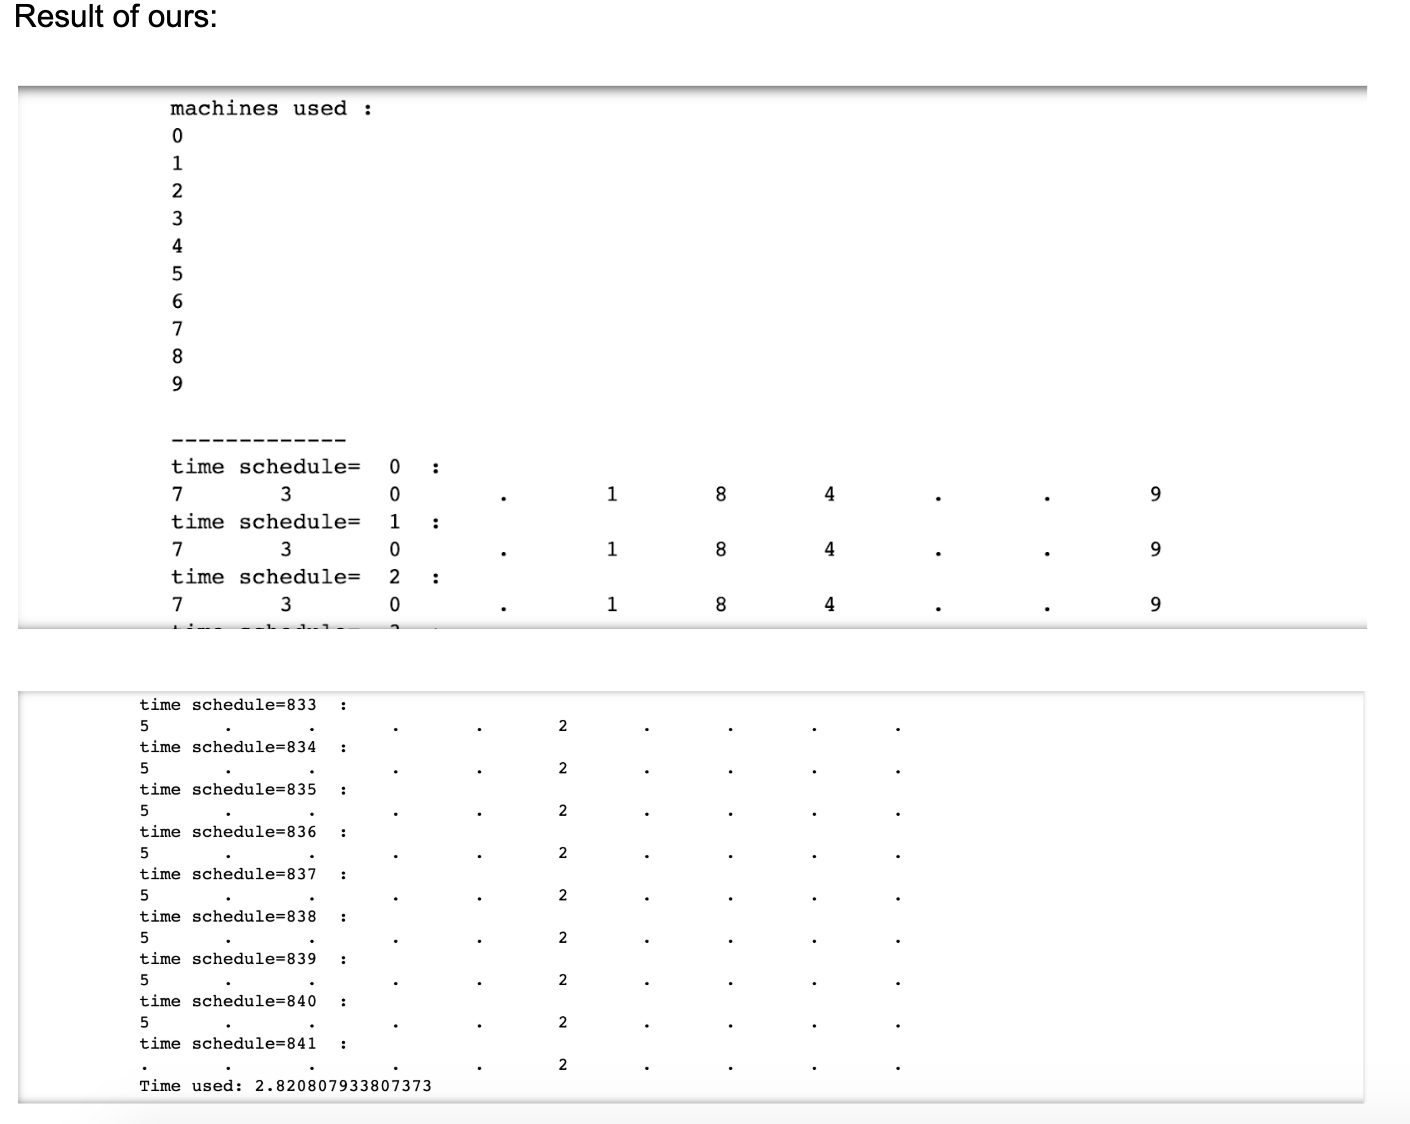
\includegraphics[width=4in]{img/sat.png}
\caption{10x10 testing result of our Z3-tool}
\end{figure}


By testing the data set 6x6, 8x8, 10x10, we learn that our Z3-tool can generate same
answer as Google-OR-tool.(\*Note that our schedule length start with 0 while
Google-OR-tool start with 1, therefore our result will be 1 unit time less than
google's) However, our performance is not as good as Google's. While the data set
comes to 15x15, our tool seems will run forever(more than 15 minutes) while Google's
only run 41.51(sec). When the data set comes to 20x20, our tool will run more than 15 minutes, while Google's only run 93.17(sec).      

\begin{figure}[H]
\centering
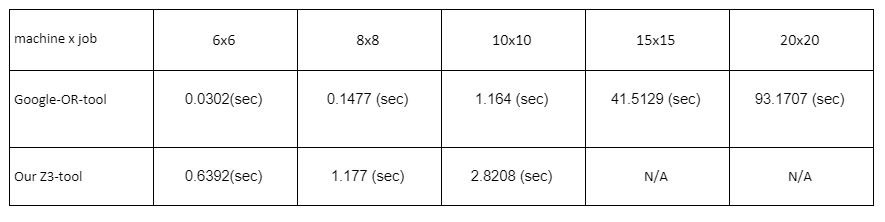
\includegraphics[width=6in]{img/4.PNG}
\caption{Result Table}
\end{figure}